\documentclass[11pt]{article}
\usepackage{amsmath,amssymb}
\usepackage{graphicx}
\usepackage{booktabs}
\usepackage[margin=1in]{geometry}
\usepackage{hyperref}
\providecommand{\tightlist}{\setlength{\itemsep}{0pt}%
  \setlength{\parskip}{0pt}}
\emergencystretch=2em

\title{Tuning-Free Continual Adaptation of Frozen Language Models via
Write-Protected Contextual Memory}
\author{Anonymous}
\date{}

\begin{document}
\maketitle
\begin{center}\rule{0.5\linewidth}{0.5pt}\end{center}

\begin{abstract}
Continual adaptation of large language models to shifting domains typically relies on gradient-based low-rank adapters (LoRA), which require per-model learning-rate tuning and incur VRAM costs that grow with batch size and model scale through retained activations and optimizer state. We attach a backpropagation-free adapter --- a block-diagonal recursive least-squares readout over spline-expanded frozen features, coupled to a write-protected contextual memory --- to GPT-2 family models (124M/355M/774M) and OPT-1.3B on a single-pass domain-return classification stream. Across scales and families, the adapter's return-onset error stays flat (0.15--0.24) while identically-configured online LoRA collapses outside a narrow learning-rate window that shifts with model size and family (divergence at lr=1e-3 on 355M/774M/1.3B, no learning at 1e-5, competitive accuracy only at 1e-4). On a 6GB device with frozen gpt2-large, LoRA's peak memory exceeds the physical wall at batch 4 and reaches 9.2GB at batch 8, while the adapter remains under the wall at batch 32 (5.1GB) with \(\sim 400\)KB of feature-space state independent of model size; on a 16GB T4 with frozen OPT-1.3B the same divergence repeats --- LoRA reaches 12.0GB at batch 32 and OOMs at batch 64 where the adapter uses 8.4GB. Tuning-free, forward-only adaptation is feasible where gradient methods cannot be tuned or cannot fit. (Speed comparison is reported only as a scoped lower bound --- update-path vs full training-step --- not a headline claim.)

\end{abstract}

\section{Introduction}\label{introduction}

\begin{quote}
Continual adaptation of large language models (LLMs) to shifting data distributions is typically addressed via gradient-based parameter-efficient fine-tuning (PEFT) methods, such as LoRA. While effective in offline settings, these methods face two fundamental bottlenecks in streaming, resource-constrained environments: (1) they require careful, model-specific learning rate tuning, where a suboptimal choice leads to catastrophic divergence or failure to learn; and (2) they incur substantial VRAM overhead due to the retention of backward-pass activations and optimizer states, which scales unfavorably with batch size and model parameters.

We propose a fundamentally different approach: a backpropagation-free, tuning-free adapter based on block-diagonal recursive least squares (RLS) coupled with write-protected contextual memory, operating entirely in the frozen feature space of the LLM. Because RLS is a second-order method, it possesses no step-size hyperparameter, eliminating the need for learning rate tuning. Furthermore, by strictly enforcing a forward-only, predict-before-update regime, our adapter avoids building a gradient graph, keeping peak VRAM dependent only on transient feature activations, not on model scale or optimizer state.

In this work, we demonstrate this mechanism on a single-pass domain-return classification stream using the GPT-2 family (124M to 774M parameters). We show that while identically configured online LoRA collapses outside a narrow, scale-dependent learning rate window, our adapter maintains stable return-onset error (0.18--0.24) across all scales. Finally, we empirically map the VRAM divergence on a 6GB device, showing that the adapter remains well within hardware limits even at large batch sizes, whereas the gradient-based baseline exceeds physical memory and incurs severe spill-overhead.
\end{quote}

\section{Related Work}\label{related-work}

\begin{quote}
\textbf{Parameter-Efficient Fine-Tuning (PEFT).} Methods like LoRA {[}Hu et al., 2021{]} and adapters {[}Houlsby et al., 2019{]} reduce trainable parameters but remain fundamentally gradient-based. They require backward passes, retaining activations in memory, and optimizer states (e.g., Adam), making their VRAM footprint structurally tied to batch size and sequence length, regardless of the low rank.

\textbf{Continual Learning without Replay.} Catastrophic forgetting is often mitigated via regularization (EWC, SI) or architectural isolation. However, these typically assume access to gradient signals or stored data buffers. Our work aligns with memory-based continual learning but operates strictly under single-pass, no-replay, and no-gradient constraints.

\textbf{Gradient-Free and Local Learning.} Reservoir computing and online RLS have long provided efficient, forward-only adaptation for time-series prediction. We extend this paradigm to frozen LLM feature streams, demonstrating that second-order, local update rules can provide robust, tuning-free adaptation where first-order gradient descent is either too fragile to tune or too expensive to fit.
\end{quote}

\section{Method}\label{method}

\begin{figure}[t]
\centering
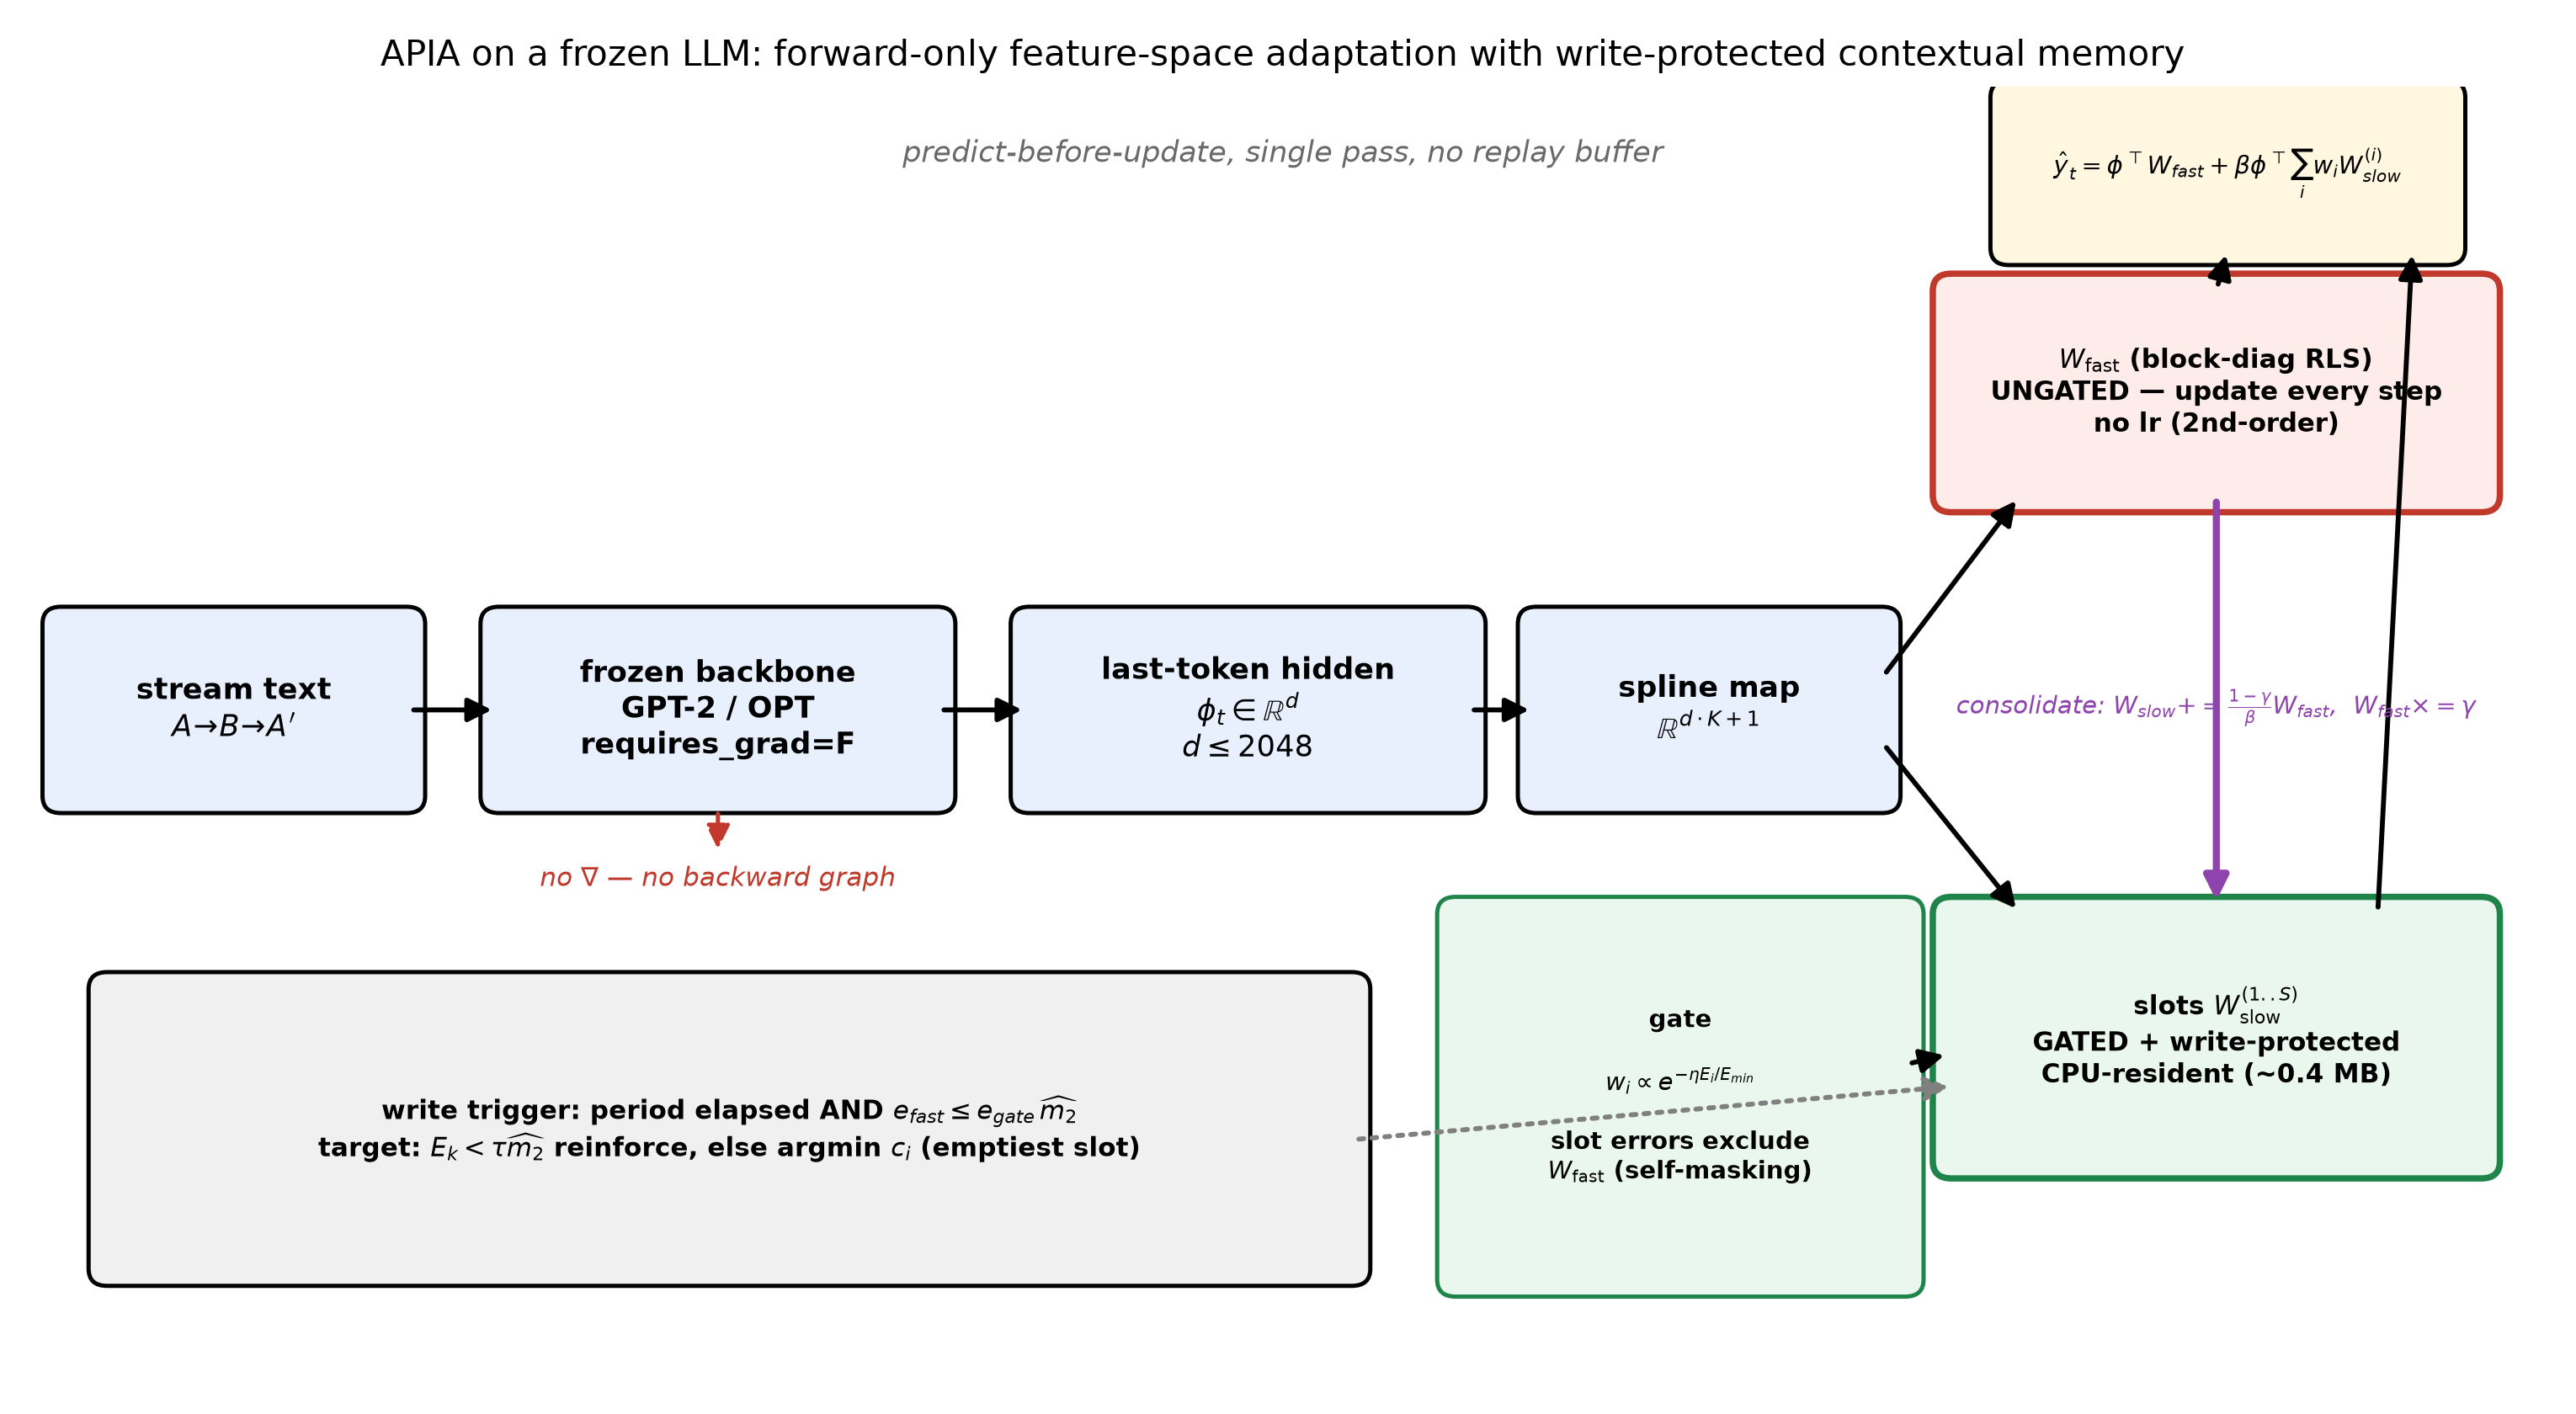
\includegraphics[width=\columnwidth]{fig1_architecture_p2.png}
\caption{Architecture. A frozen backbone (GPT-2 or OPT, $\texttt{requires\_grad}=\mathrm{False}$, $\texttt{no\_grad}$) emits a last-token feature $\phi_t$; a fixed cubic B-spline map lifts it to $\mathbb{R}^{d\cdot K+1}$. The ungated fast channel $W_{\mathrm{fast}}$ (red) is a block-diagonal RLS updated every step --- no learning rate, no backward graph. The gated slow slots $W_{\mathrm{slow}}^{(i)}$ (green) receive a $(1{-}\gamma)/\beta$-scaled copy of $W_{\mathrm{fast}}$ only when the write trigger fires and the target passes write protection. The whole learning state is CPU-resident.}
\label{fig:arch}
\end{figure}

\begin{quote}
Our approach attaches a backpropagation-free, stateful adapter to the frozen representations of a pre-trained language model. The architecture strictly enforces a predict-before-update, single-pass constraint, ensuring that no gradient graph is ever constructed through the backbone.

\textbf{3.1 Frozen backbone and feature stream.} The base model weights are frozen (\texttt{requires\_grad=False}), and inference is executed under \texttt{torch.no\_grad()}. For each incoming sequence we extract the last-token hidden state of the final transformer block, yielding \(\phi_t\) \(\in\) \(\mathbb{R}^d\), d \(\in\) \{768, 1024, 1280\} for the GPT-2 family. The adapter operates exclusively in this feature space: because the interface dimension d is bounded and independent of backbone parameter count, the learning problem is structurally identical whether features come from a 124M or a 774M model. In the reported experiments features are standardized with stream-wide statistics; online deployment requires a streaming mean/variance estimator (Sec. 5). An optional fixed random projection (768\(\to 100\), tanh) was found to bottleneck probe accuracy (90.25\%\(\to 81.25\)\%) and is not used in the main experiments.

\textbf{3.2 Spline expansion and block-diagonal RLS.} To capture non-linear boundaries without backpropagation, \(\phi_t\) is expanded by a fixed per-dimension cubic B-spline basis (\(\mathbb{R}^d\) \(\to\) \(\mathbb{R}^{d\cdot K+1}\), K=10, plus bias). The expanded representation feeds a block-diagonal recursive least-squares readout. RLS is second-order: the update magnitude is set implicitly by the inverse-covariance blocks P, so there is no step-size hyperparameter to tune. The block-diagonal approximation keeps per-step cost at \(O(d\cdot K^2)\) and the full learning state (\(W_{\mathrm{fast}}\), P) at \(\sim 250\)--410KB on CPU --- independent of backbone size.

\textbf{3.3 Write-protected contextual memory.} The readout splits into a fast, ungated channel (\(W_{\mathrm{fast}}\), updated every step on the gated residual) and N gated slow slots (\(W_{\mathrm{slow}}^{(i)}\)). Consolidation runs periodically (every \texttt{consolidate\_every} steps) but only fires when the short-term fast error is stable, \(e_{\mathrm{fast}}\) \(\leq\) \(e_{\mathrm{gate}}\)\(\cdot\)\(\widehat{m_2}\), where \(\widehat{m_2}\) is an online estimate of \(\mathbb{E}[y^2]\) --- a trigger that must be rescaled to the task's error baseline (\(e_{\mathrm{gate}}\)=1.0 for 0/1 labels; the regression-calibrated 0.5 nearly disables consolidation on classification). Write protection then selects the target: if the best-matching slot's context-match error \(E_i = \|y_t - \beta\,\phi_t^\top W_{\mathrm{slow}}^{(i)}\|^2\) --- computed \emph{excluding} \(W_{\mathrm{fast}}\) to avoid self-masking --- satisfies \(E_{\min}\) \textless{} \(\tau\)\(\cdot\)\(\widehat{m_2}\), that slot is reinforced; otherwise the write goes to the least-consolidated slot (\(\arg\min_i c_i\)), so heavily consolidated memories are not overwritten by transient noise. At saturation the `refuse' policy skips the write entirely. The transfer preserves prediction continuity: \(W_{\mathrm{slow}}^{(k)}\) \(\leftarrow\) \(W_{\mathrm{slow}}^{(k)}\) + \((1-\gamma)/\beta \cdot W_{\mathrm{fast}}\), then \(W_{\mathrm{fast}}\) \(\leftarrow\) \(\gamma\)\(\cdot\)\(W_{\mathrm{fast}}\) (\(\gamma\)=0.1).

\textbf{3.4 Gate time constant.} The slot-match EMA must be much faster than the regime-transition window: the default \(\alpha_{\mathrm{ema}}\)=0.01 (\(\sim 100\)-step lag) leaves a stale slot active at domain return and poisons the onset; \(\alpha_{\mathrm{ema}}\)=0.05 with sharper gating (\(\eta\)=5.0) reduced return-onset error 0.30\(\to 0.23\) on raw-768 features.

\textbf{3.5 Why no lr / why VRAM-flat (independent properties).} No-lr follows from RLS being second-order (update magnitude set by P). VRAM-flat follows from forward-only execution: activations are transient and freed per batch --- peak \(\approx\) weights + O(B\(\cdot\)d\(\cdot\)L) transient, not weights + activations + grads + 2\(\times\)optimizer state. Both share the root of local forward-only learning but are NOT causally chained.
\end{quote}

\section{Experiments}\label{experiments}

\subsection{Experimental Setup}\label{experimental-setup}

\begin{quote}
\textbf{Tasks and protocol.} We evaluate continual adaptation on a single-pass, domain-return classification stream built from 20 Newsgroups: phase 1 learns domain A (sci.space vs rec.sport.baseball, 600 samples), phase 2 domain B (comp.graphics vs talk.politics.misc, 600 samples), phase 3 returns to fresh samples of domain A' (400 samples). Strict online constraints throughout: single pass, predict-before-update, no replay buffer, no offline batch training.

\textbf{Models and baselines.} The adapter attaches to the frozen GPT-2 backbone (124M/355M/774M; \texttt{requires\_grad=False}, \texttt{torch.no\_grad()} inference). The learning boundary is strict: the backbone provides pure inference features (last-token hidden state, d \(\in\) \{768, 1024, 1280\}) and all adaptation happens feature-space-side. Two arms: (i) \textbf{APIA} --- block-diagonal RLS over spline-expanded features + write-protected contextual memory (S=3 slots), learning state \(\approx 250\)--410KB on CPU, independent of model scale; (ii) \textbf{online LoRA} --- r=8 on \texttt{c\_attn}/\texttt{c\_proj}, AdamW, updated per sample on the same stream.

\emph{Feature normalization caveat: reported experiments standardize with stream-wide statistics; edge deployment requires a streaming estimator (Sec. 5).}

\textbf{Metrics.} Phase-end and return-onset error (first 100 samples of A' --- adaptation speed and forgetting); peak VRAM via \texttt{torch.cuda.max\_memory\_allocated()}; per-step latency.

\textbf{Hardware.} GPT-2-scale runs on an RTX 3060 Laptop (6GB) deliberately below the wall; the 1.3B extension (OPT-1.3B) targets a 16GB Kaggle T4 to re-test divergence at a higher ceiling.
\end{quote}

\subsection{Finding 1 --- scale-stability}\label{finding-1-scale-stability}

\begin{quote}
Table~\ref{tab:table1} reports return-onset error for both arms across the GPT-2 family, extended to a different model family (OPT-1.3B, d=2048) on a 16GB T4. With identical configuration --- no learning rate exists to retune --- the adapter's onset error stays within 0.15--0.24 from 124M to 1.3B parameters. Identically configured online LoRA (r=8, lr=1e-3, a setting that works well at 124M) degrades to 0.46--0.52 on the larger models, i.e., near-chance. The adapter's learning dynamics live entirely in feature space (\(\phi_t\) \(\in\) \(\mathbb{R}^d\)): the readout and memory see the same dimensionality regardless of how many parameters produced the features, so scale changes the backbone, not the learning problem.
\end{quote}

\begin{table}[t]
\centering\small
\begin{tabular}{lllll}
\toprule
Model & Params & APIA onset & LoRA (lr=1e-3) & LoRA status \\
\midrule
GPT-2 & 124M & 0.23 & 0.19 & optimal \\
GPT-2 Medium & 355M & 0.18 & 0.49 & diverged \\
GPT-2 Large & 774M & 0.20 & 0.52 & diverged \\
OPT-1.3B (fp16, T4) & 1.3B & 0.15 & 0.46 & diverged \\
\bottomrule
\end{tabular}

\caption{Return-onset error across scales and families. Identical configuration throughout; the adapter has no lr to retune. OPT-1.3B row measured on a 16GB T4 (fp16).}
\label{tab:table1}
\end{table}

\subsection{Finding 2 --- lr fragility}\label{finding-2-lr-fragility}

\begin{quote}
Section 4.2's LoRA collapse is not a fundamental failure of low-rank adaptation --- it is a tuning failure. Table~\ref{tab:table2} sweeps lr \(\in\) \{1e-3, 1e-4, 1e-5\} on gpt2-medium and gpt2-large. On medium, lr=1e-3 diverges (0.49 onset), lr=1e-4 attains 0.09, and lr=1e-5 never learns (0.51). On large the pattern repeats: lr=1e-3 diverges (0.52), lr=1e-4 attains the best onset of the whole study (0.06), and lr=1e-5 only partially learns within the stream (0.32 onset, still improving at 0.18 by phase end). Two observations matter for deployment: (i) the usable window is narrow --- a factor of 10 in either direction destroys or cripples the run; (ii) the window's position is not predictable from the smaller model --- 1e-3 is optimal at 124M and fatal at 355M+. In a streaming setting there is no held-out pass for a grid search; the stream arrives once. The adapter sidesteps the question entirely: RLS has no step-size parameter, and the identical configuration that runs at 124M runs at 774M.
\end{quote}

\begin{table}[t]
\centering\small
\begin{tabular}{lllll}
\toprule
Model & lr & Onset err & Phase-end & Observation \\
\midrule
GPT-2 Medium & 1e-3 & 0.49 & 0.53 & divergence \\
GPT-2 Medium & 1e-4 & \textbf{0.09} & 0.06 & optimal \\
GPT-2 Medium & 1e-5 & 0.51 & 0.51 & no learning \\
GPT-2 Large & 1e-3 & 0.52 & 0.51 & divergence \\
GPT-2 Large & 1e-4 & \textbf{0.06} & 0.02 & optimal (unpredictable) \\
GPT-2 Large & 1e-5 & 0.32 & 0.18 & partial/slow \\
OPT-1.3B (T4) & 1e-3 & 0.46 & 0.60 & divergence (cross-family) \\
OPT-1.3B (T4) & 1e-4 & \textbf{0.05} & 0.04 & optimal \\
\bottomrule
\end{tabular}

\caption{Learning-rate fragility of online LoRA (r=8). The viable window is narrow and shifts with scale; the pattern repeats on a different model family (OPT-1.3B).}
\label{tab:table2}
\end{table}

\begin{quote}
On OPT-1.3B the memory arm also transfers: \texttt{apia\_ctxmem} reaches 0.15 return-onset vs 0.22 for the memoryless \texttt{apia\_block} (6 consolidations over the stream), confirming that write-protected consolidation operates on frozen features from a second model family without retuning.
\end{quote}

\begin{figure}[t]
\centering
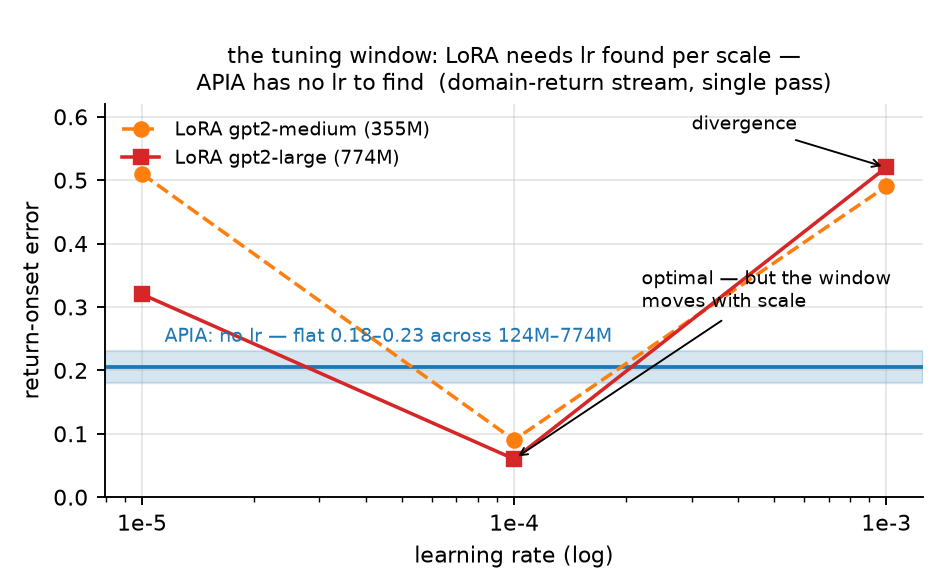
\includegraphics[width=\columnwidth]{fig2_lr_sweep.png}
\caption{Learning-rate fragility (return-onset error vs lr, log scale). LoRA forms a U-shape that bottoms near lr=1e-4 on both model sizes but diverges at 1e-3 and fails to learn at 1e-5; the APIA band is flat because RLS has no step size.}
\label{fig:lrsweep}
\end{figure}

Honest note. tuned LoRA beats APIA decisively on accuracy (0.05--0.09 vs 0.15--0.23 onset, now including OPT-1.3B) --- the gap persists across families, and this must be stated, not hidden. The claim is tunability + memory, not accuracy.

\subsection{Finding 3 --- VRAM wall}\label{finding-3-vram-wall}

\begin{quote}
Fig.~\ref{fig:vram} changes the axis from accuracy to hardware cost. On a 6GB device running frozen gpt2-large (seq-128), peak VRAM for the forward-only adapter grows from 3,243MB at batch 1 to 5,132MB at batch 32 --- transient activations freed under \texttt{no\_grad}, plus \(\sim 400\)KB of feature-space state on CPU. The LoRA arm (fwd+bwd+AdamW) reaches 6,191MB at batch 4 --- already past the device's physical 6,144MB --- and requests 9,159MB at batch 8, forcing \(\sim 4\)GB of spill into shared RAM where step time inflates 2.2\(\times\) (575\(\to 1\),267ms) from memory pressure, not compute. Note this is the independent property, not a corollary of Sec.~4.3: even a perfectly tuned LoRA pays this memory bill, because retained activations and optimizer state are structural to gradient descent, not to any particular lr.
\end{quote}

\begin{table}[t]
\centering\small
\begin{tabular}{lllll}
\toprule
Batch & APIA peak & LoRA peak & LoRA step & Status \\
\midrule
1 & 3,243 & 3,989 & 268 ms & fits \\
4 & 3,425 & \textbf{6,191} & 575 ms & exceeds wall \\
8 & 3,670 & \textbf{9,159} & 1,267 ms & $\sim$4GB spill \\
32 & 5,132 & --- & --- & APIA still fits \\
\bottomrule
\end{tabular}

\caption{Peak VRAM on a 6,144MB device (frozen gpt2-large, seq-128). APIA grows only via transient forward activations; the $\sim 400$KB learning state is CPU-resident.}
\label{tab:table3}
\end{table}

\begin{quote}
The wall moves, but does not disappear. Repeating the same scan on a frozen OPT-1.3B backbone (fp16, weights 2,632MB) on a 16GB T4, the adapter grows 2,731\(\to 8\),406MB from B=1 to B=64 --- under half the device at every point. The LoRA arm reaches 12,023MB at B=32 and OOMs at B=64; the LoRA/APIA peak ratio grows monotonically with batch (1.08\(\times\) \(\to\) 2.18\(\times\)). More headroom delays the divergence; it does not remove it, because the retained-activation bill is proportional to batch while the forward-only cost is not.
\end{quote}

\begin{figure}[t]
\centering
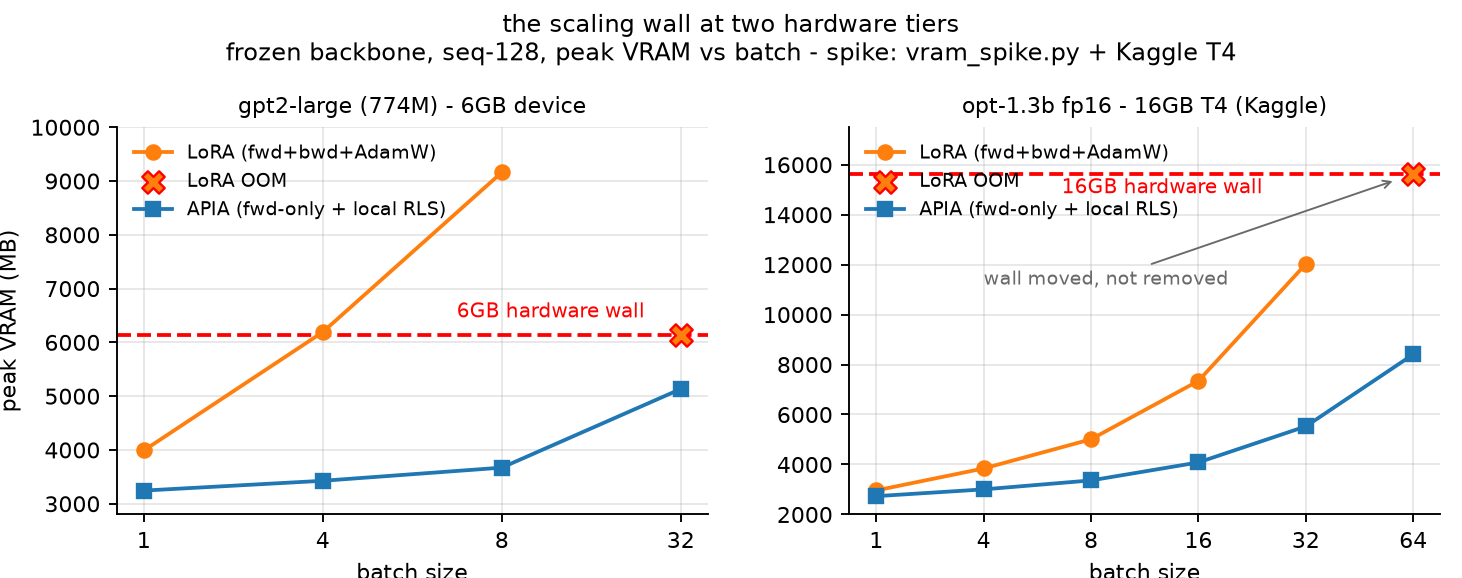
\includegraphics[width=\columnwidth]{fig_vram_dual.png}
\caption{Peak VRAM vs batch at two hardware tiers. Left: 6GB device, frozen gpt2-large --- LoRA crosses the wall at B=4 and spills $\sim$4GB at B=8. Right: 16GB T4, frozen OPT-1.3B --- same divergence delayed, not removed (LoRA OOM at B=64; adapter at 8.4GB). X marks the measured OOM point.}
\label{fig:vram}
\end{figure}

\begin{table}[t]
\centering\small
\begin{tabular}{lllll}
\toprule
Batch & APIA peak & LoRA peak & LoRA/APIA & Status \\
\midrule
1 & 2,731 & 2,961 & 1.08$\times$ & both fit \\
4 & 3,002 & 3,839 & 1.28$\times$ & both fit \\
8 & 3,361 & 5,008 & 1.49$\times$ & both fit \\
16 & 4,082 & 7,345 & 1.80$\times$ & both fit \\
32 & 5,523 & 12,023 & 2.18$\times$ & LoRA near wall \\
64 & 8,406 & \textbf{OOM} & --- & LoRA $>$16GB wall \\
\bottomrule
\end{tabular}

\caption{Peak VRAM on a 15,636MB T4 (frozen OPT-1.3B fp16, seq-128, Kaggle). Same divergence at the higher ceiling: LoRA OOMs at B=64 while the adapter uses $\sim 54$\% of the device.}
\label{tab:table4}
\end{table}

Timing caveat. scopes differ (feature-space RLS vs full fwd+bwd+opt) --- speed gap is a lower bound, not a headline; memory divergence is the structural claim. On the T4 the scope gap is explicit: LoRA runs 26--32ms/sample fwd+bwd+opt at all measured batch sizes while APIA amortizes to 0.3ms/sample at B=64.

\section{Discussion}\label{discussion}

\begin{quote}
The empirical results establish a unified message: local, forward-only learning possesses two independent structural advantages over gradient-based adaptation in streaming environments. First, because RLS is second-order, it has no step-size hyperparameter, yielding scale-stable accuracy without per-model tuning. Second, because it requires no backward pass, its adaptation memory scales strictly with the feature dimension d, not the backbone size, allowing it to operate beneath hardware VRAM walls where forward+backward+optimizer pipelines fail. These are independent properties sharing a common root (forward-only execution), not a causal chain.

\textbf{Limitations.} We state the boundaries of this proof-of-concept transparently:
1. \textbf{Accuracy vs.~tunability trade-off:} when perfectly tuned (lr=1e-4), LoRA reaches 0.09/0.06/0.05 onset on medium/large/OPT-1.3B vs the adapter's 0.18/0.20/0.15 --- the gap persists across families. We explicitly trade peak accuracy for elimination of tuning fragility and guaranteed memory bounds.
2. \textbf{Feature normalization:} current experiments use stream-wide statistics; true online deployment requires a streaming mean/variance tracker.
3. \textbf{Scope:} accuracy claims cover the GPT-2 family (d \(\leq\) 1280) plus OPT-1.3B fp16 (d = 2048) on a single binary domain-return stream; broader tasks and further families remain open. The LoRA baseline is one r=8 config (rank/schedule variants unexplored).
4. \textbf{Gate latency:} the slot-match EMA imposes a lag of order 1/\(\alpha_{\mathrm{ema}}\) steps after each regime shift; at the default 0.01 the stale slot poisons the onset (measured 0.30\(\to 0.23\) with \(\alpha_{\mathrm{ema}}\)=0.05).

\textbf{Future work.} Both the 1.3B wall (Table~\ref{tab:table4}) and the 1.3B accuracy arm (Tables~\ref{tab:table1}--\ref{tab:table2}) are now measured: next steps are still larger models (2.7B/6.7B) where fp16 weights alone approach the 16GB ceiling, quantized (int8/int4) RLS to shrink adapter state, dynamic slot allocation on severe context mismatch, multi-seed robustness, and direct mapping of the \(O(d\cdot K^2)\) update to FPGA/analog hardware.
\end{quote}

\section{Conclusion}\label{conclusion}

\begin{quote}
We have demonstrated that tuning-free, forward-only adaptation is a viable and structurally superior alternative to gradient-based adapters in streaming, hardware-constrained settings. By operating exclusively in the frozen feature space with block-diagonal RLS and write-protected contextual memory, our method eliminates the learning rate tuning burden and decouples adaptation memory from model scale. Empirical results on the GPT-2 family --- extended to OPT-1.3B on a 16GB T4 --- confirm that while online LoRA is highly fragile to learning rate choices that shift with model size and family, our adapter remains stable. Furthermore, on both a 6GB device and a 16GB accelerator, the adapter avoids the VRAM wall that forces gradient-based methods into spill overhead or outright OOM. This establishes a clear path toward deployable, lifelong learning for large models at the edge.
\end{quote}

\begin{center}\rule{0.5\linewidth}{0.5pt}\end{center}

\section*{References}
\begin{itemize}\tightlist
\item E.~J. Hu et al., ``LoRA: Low-Rank Adaptation of Large Language
  Models,'' \emph{ICLR}, 2022. arXiv:2106.09685.
\item N. Houlsby et al., ``Parameter-Efficient Transfer Learning for
  NLP,'' \emph{ICML}, 2019.
\item J. Kirkpatrick et al., ``Overcoming catastrophic forgetting in
  neural networks,'' \emph{PNAS} 114(13), 2017.
\item F. Zenke, B. Poole, S. Ganguli, ``Continual learning through
  synaptic intelligence,'' \emph{ICML}, 2017.
\item H. Jaeger, ``The `echo state' approach to analysing and training
  recurrent neural networks,'' GMD Report 148, 2001.
\item S. Haykin, \emph{Adaptive Filter Theory}, 5th ed., Pearson, 2014
  (recursive least squares).
\item A. Radford et al., ``Language models are unsupervised multitask
  learners,'' OpenAI Tech. Report, 2019 (GPT-2).
\item S. Zhang et al., ``OPT: Open pre-trained transformer language
  models,'' arXiv:2205.01068, 2022.
\end{itemize}

\end{document}
